\subsection{Controls on the acquired center--slope geometry}
\label{app:geometry-controls}

These controls distinguish readout optimization from changes to the features
themselves. They use the primary mixed-sine target, total width~512, five
paired seeds, and the grids and error metric in
Appendix~\ref{app:slope-experiments}. A source optimizer is the optimizer that
learned the features; \emph{every iterative follow-up readout uses Adam},
including readouts of GD-acquired features.

\paragraph{Protocol.}
Readout restarts freeze the features and run two million additional updates
from zero readout and zero moments. Each dictionary tests rates
$\{10^{-5}/3,10^{-5},10^{-4},10^{-3},0.002,0.01,0.1,0.3\}$ under constant
and full-horizon cosine schedules. One complete recipe is selected per
dictionary by final validation error; no earlier checkpoint replaces the
endpoint. These additional updates diagnose feature quality rather than
matching end-to-end training cost. Direct FP64 SVD fits use a relative
singular-value cutoff of $10^{-12}$, with $10^{-14}$ and $10^{-16}$ as
sensitivity checks. Reported errors are recomputed on the 8,192-point dense
grid. Independent columnwise reconstruction verifies the saved final fits;
on this machine it changes accumulation order, not precision. No truncated
fit is interpreted as a certified capacity floor.

\paragraph{Readout access improves as features are acquired.}
For Adam-acquired features, median restart error decreases from $0.808$ at
initialization to $0.0408$ at 200k, $0.0305$ at 600k, and $0.00250$ at two
million joint updates. For GD-acquired features, the corresponding errors
are $0.808$, $0.276$, $0.256$, and $0.251$. At the final Adam features,
restart error $0.002501$ nearly matches the original joint endpoint
$0.002509$. The direct fit reaches $0.002407$, with median coefficient
$L^2$ norm $1.12\times10^7$; cutoff $10^{-14}$ gives $0.002385$ and norm
$8.22\times10^8$. These fits give little evidence that optimizing this
particular frozen readout more accurately would close the gap to the
supplied uniform dictionary. For final GD features, the direct-fit median
is $0.217$, below the restart's $0.251$ but still far from high precision.

\begin{figure}[t]
 \centering
 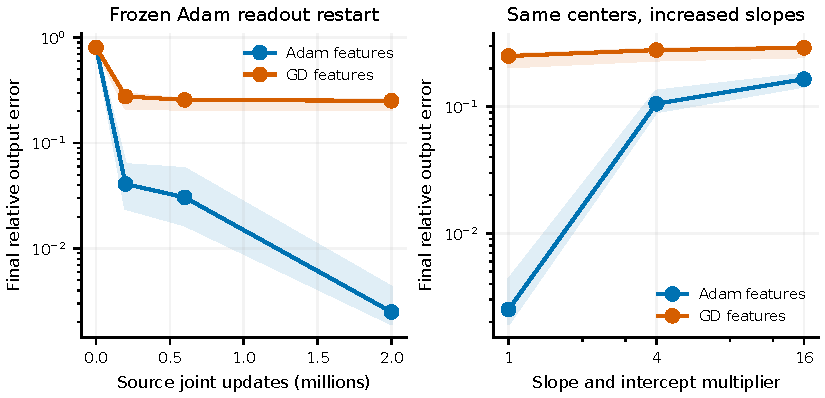
\includegraphics[width=\linewidth]{output/diagnostics/section34_long_horizon/geometry_2m/feature_access_assays.pdf}
 \caption{Readout access through acquired features. Source labels identify
 the joint optimizer; all follow-up readouts use Adam for two million
 additional updates. Feature snapshots and final slope interventions use
 the same candidate recipes and final-validation selection rule. The target
 is the primary mixed sine, with five paired seeds.}
 \label{fig:geometry-readout-controls}
\end{figure}

\paragraph{Steepening can reduce accuracy.}
Multiplying both $a_j$ and $b_j$ in $\tanh(a_jx+b_j)$ by four or sixteen
preserves its center $-b_j/a_j$. For final Adam features, these changes
increase median restart error to $0.1056$ and $0.1652$, respectively;
median paired increases are $42.2\times$ and $66.0\times$.
Direct fits yield the same medians at cutoffs $10^{-12}$ and $10^{-14}$,
with much smaller coefficient norms than the unscaled fits. For final GD
features, restart medians increase to $0.280$ and $0.292$, although
direct-fit medians decrease to $0.205$ and $0.156$.
A slope change therefore affects both the approximation and access to it.
The new dictionary need not contain the old span: steeper features can lose
a useful approximation. This is not a monotone intervention proving that
larger slopes always improve a learned model.

\paragraph{Isolated geometry replacements do not restore high precision.}
Two further controls use the final unscaled dictionaries. One places their
exact signed slopes on the uniform reference centers, with one predeclared
permutation per source optimizer and seed. The other preserves learned
centers and signs but sets every slope magnitude to $\gamma=0.25/h$.
Neither adds neurons. Their direct-fit medians are respectively $0.1146$
and $0.07885$ for Adam-acquired features, and $0.3735$ and $0.2659$ for
GD-acquired features. At cutoff $10^{-14}$, Adam's medians are unchanged;
GD's are $0.3384$ and $0.2651$. Actual matched Adam readout training reaches
medians $0.1422$ and $0.07929$ for Adam-acquired sources, and $0.4734$ and
$0.2724$ for GD-acquired sources. Neither isolated replacement restores the
original Adam geometry's accuracy. Six of twenty selected recipes lie at
the already expanded rate-grid boundary; this limits claims about optimal
tuning. No further expansion is performed.

\begin{figure}[t]
 \centering
 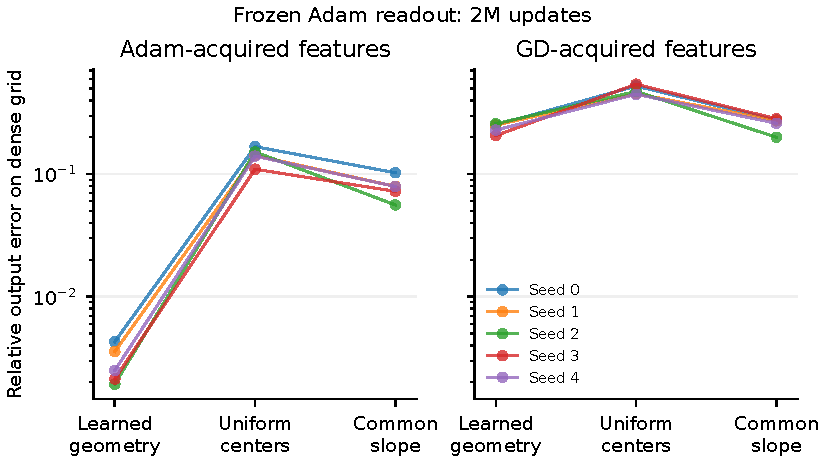
\includegraphics[width=\linewidth]{output/diagnostics/section34_long_horizon/geometry_2m/paired_intervention_errors.pdf}
 \caption{Executed geometry-replacement controls, paired by seed. Categories
 show the original learned geometry, uniform centers with its learned
 slopes, and its learned centers with common slope magnitude $0.25/h$.
 Panels distinguish the source joint optimizer. Every dictionary, including
 the original baseline, receives two million additional frozen Adam updates
 after two million joint updates; final validation error selects a complete
 recipe. The vertical axis is relative error on the dense resolution-check
 grid. Neither replacement improves median accuracy.}
 \label{fig:geometry-replacement-controls}
\end{figure}

Although 97.85--99.02\% of Adam's learned centers lie inside the interval,
the 512 centers occupy only 41--49 distinct locations after rounding to
12 decimal places. Most coalesced centers belong to nearly zero-slope
units. Interior units with $h|a_j|\ge0.01$ have 35--37 distinct centers,
occupying 27--29 of 32 equal domain bins. Their coverage is much better
than unweighted center quantiles suggest. GD has only 5--7 such interior
units, occupying 3--7 bins. These thresholds describe the measured geometry;
they do not define a theorem assumption or an invariant active-neuron count.
Assigning a common large slope reactivates many nearly coincident features
and need not supply 512 distinct useful directions.

The controls support interpreting the joint-training gap through the
acquired center--slope geometry, rather than a single slope statistic.
The uniform-dictionary theorem quantifies slope-dependent readout delay
under its stated geometry; these controls neither extend it to arbitrary
joint training nor prove an Adam convergence law.

\paragraph{Acquisition continues over the longer horizon.}
The independently checked five-million-update Adam comparison selects cosine
decay from rate $0.05$ and reaches median dense error $0.001815$, a 27.7\%
reduction from $0.002509$ at two million updates. These are fresh runs with
decay over their respective full horizons; not every seed improves.
Its seeds have 50--56 neurons with $h|a_j|\ge0.01$, versus 36--43 at two
million updates, and 41--45 with $h|a_j|\ge0.1$, versus 25--29.
The $99$th-percentile slopes reach $0.233$--$0.257$, but only 4--7 of
512 neurons reach $0.25$. An upper percentile near the uniform reference
does not mean the full width acquired a common slope. These counts show
continued acquisition without establishing a required count for arbitrary
geometries. Appreciably sloped interior centers occupy 28--31 of 32 bins.
For the remaining units, raw center-coalescence counts can be numerically
misleading: three seeds contain 421--457 subnormal input slopes, making
center ratios of nearly vanished features delicate. The earlier
interventions remain controls on the two-million-update source dictionaries.

Repeating the readout assays on the actual five-million-update source
features gives median error $0.00181474$ for Adam-acquired features and
$0.24209$ for GD-acquired features, compared with $0.002501$ and $0.25134$
from the two-million-update source features. Every assay still uses
\emph{two million additional Adam readout updates}, regardless of source
optimizer or horizon. At the final Adam features, the restarted readout
nearly reproduces the original joint error $0.00181482$.

Separate interventions on the five-million-update source features also
worsen accuracy. Multipliers four and sixteen give median errors
$0.09161$ and $0.13893$ for Adam-acquired features, with median paired
increases of $41.7\times$ and $69.2\times$ over their unmodified restarts.
Every seed worsens. GD-acquired features give $0.27952$ and $0.28804$,
also worse in every seed. The adverse intervention result thus persists
at the longer source horizon.

\begin{figure}[t]
 \centering
 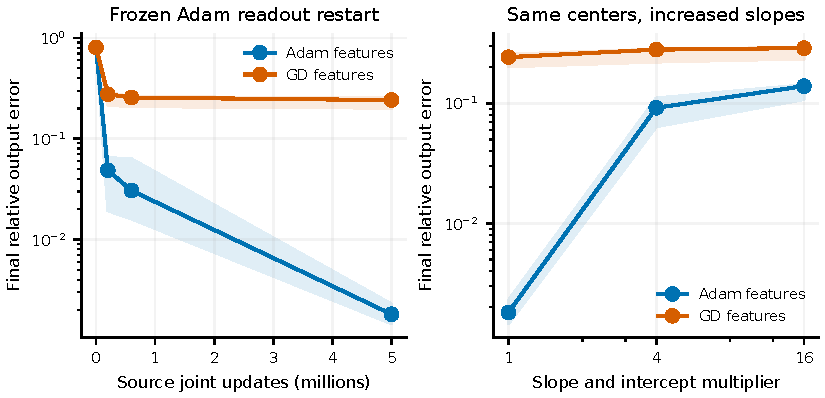
\includegraphics[width=\linewidth]{output/diagnostics/section34_long_horizon/main_5m/geometry_diagnostics/feature_access_assays_5m.pdf}
 \caption{Five-million-update source trajectories tested with two million
 additional frozen Adam updates per dictionary. Left: median dense error
 from features acquired at the indicated source update, with the five-seed
 range shaded. Right: the same readout protocol after multiplying slopes
 and intercepts of the final five-million-update features. Legends identify
 the source optimizer; all readout restarts use Adam. Earlier snapshots
 belong to these fresh full-horizon schedules, not to the previous
 two-million-update source runs.}
 \label{fig:geometry-readout-controls-five-million}
\end{figure}

Direct fits to the final five-million-update Adam features reach median
dense error $0.0018137$ at cutoff $10^{-12}$, compared with actual joint
error $0.0018148$, with median coefficient norm $1.89\times10^6$.
Cutoff $10^{-14}$ gives $0.0018119$ and norm $3.10\times10^8$; the
$10^{-16}$ cutoff does not improve the median. The longer horizon improves
both the actual output and the accuracy found by these direct fits, while
leaving little measured gain from refitting the final readout. This is not
a lower bound on the error of all possible readouts.
